\chapter{QWidgets \& Layout}

\section{QWidgets}
Applikation mit GUI = Problem-Domain + Darstellung + Interaktion \\
Bsp.: Counter = Funktionalität (inkrementieren und dekrementieren) + Fenster mit inc \& dec Buttons und der Anzeige des aktuellen Counter-Stands + Inkrementieren, wenn inc-Button gedrückt.
\textbf{Allgemeine Konzepte von GUI Frameworks} \\
\textbf{Ansicht festlegen:} Visuelle Elemente in der Benutzeroberfläche werden mittels Klassen vom GUI Framework zur Verfügung gestellt. \\
\textbf{Interaktion} mit dem Programmbenutzer -> Signals \& Slots

\subsection{QWidget Klasse}
QWidget (Widget = "Window Gadget") ist eine Basisklasse für alle anderen Qt Widgets wie bspw. QLabel, QLineEdit, QPushButton
QWidget übernimmt als Parent-Widget folgende Aufgaben:
- Anzeigen, verstecken, freigeben, sperren -> wird auch auf die Child-Widgets angewendet \\
- Weiterleiten von Ereignissen an die betroffenen Child-Widgets\\
- Memory Management \\
\begin{figure}[hb]
	\centering
\adjustbox{width=7.5cm}{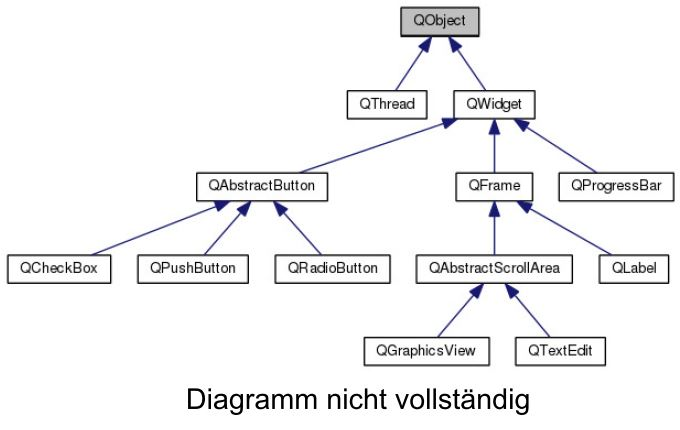
\includegraphics{Figures/qtwidgets_objekte}}
	\caption[]{Qt Vererbungen von QObject und QWidget}
\end{figure}

\section{Layout}

\begin{tabular}{|l|l|l|}
	Art & Selbst codiertes GUI & GUI-Designer (Qt Creator) \\
	Beschreibung & C++ Code für GUI Beschreibung & Interaktives Tool \\
	Vorteil & kann sich zur Laufzeit ändern & schnell zusammen "geklickt" \\
	Nachteil & aufwändig, Code selber schreiben & Nur statische Design möglich
\end{tabular}

Bei der Erstellung eines GUIs mittels WYSIWYG Editor – GUI-Designers (Qt-Creator) erfolgt die Anordnung der Widgets innerhalb eines sogenannten Formulars mit Hilfe eines interaktiven Tools. Es erfolgt eine automatische Umwandlung der Formulardaten (*.ui) in entsprechenden Programmcode mittels uic. 

\subsection{Manuelles Layout}

\begin{figure}[ht]
	\centering
	\adjustbox{width=0.8\textwidth}{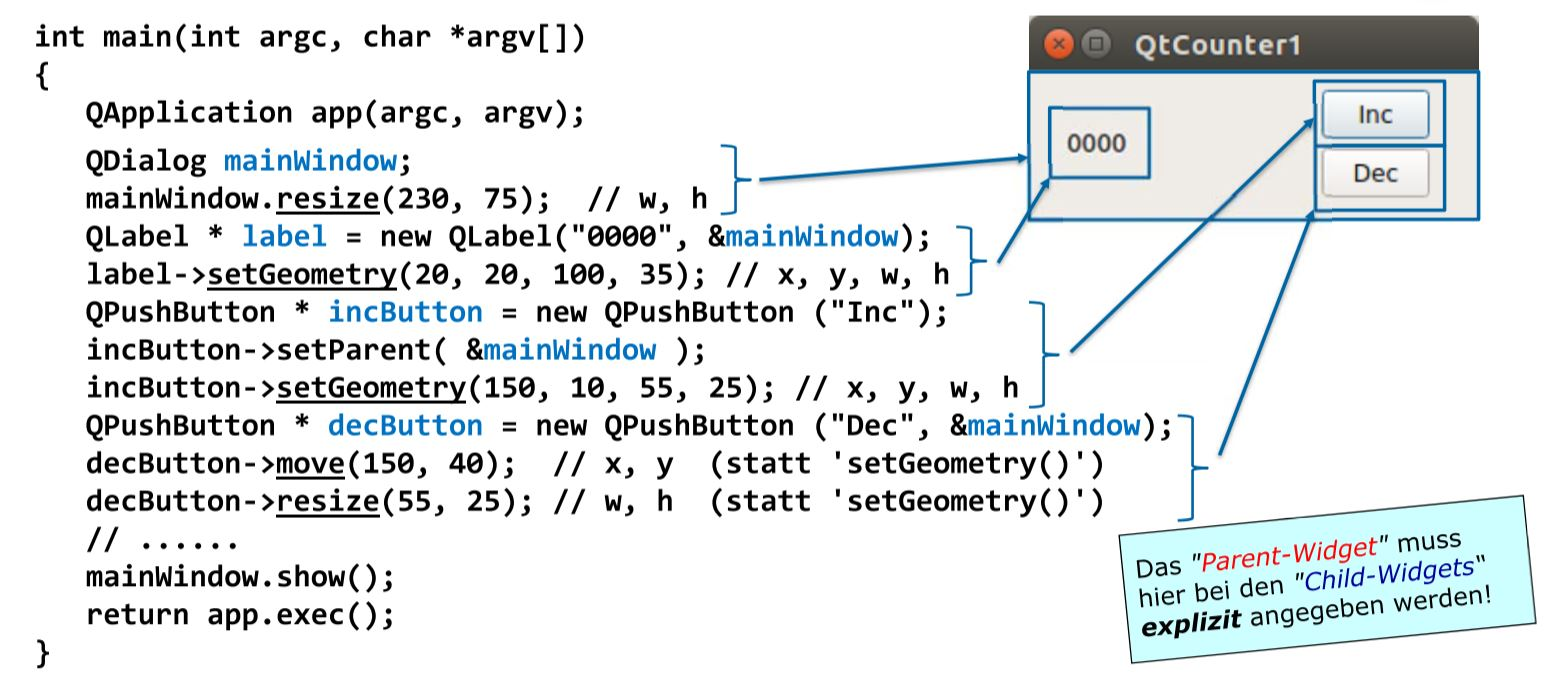
\includegraphics{Figures/Layout}}
	\caption[]{Beispeil eines manuellen Layouts}
\end{figure}

Die Positionierung erfolgt mittels eines Koordinatensystems bei dem der Ursprung (0,0) in der linken oberen Ecke ist. Die Position und Grösse wird in Pixel angegeben. Die x-Werte erhöhen sich nach rechts, während die y-Werte nach unten ansteigen. (x, y) sind die Koordinaten der linken oberen Ecke eines Widgets innerhalb eines anderen, des äusseren Widgets. w, h sind Breite und Höhe des inneren Widgets.

Methoden zur Festlegung von Position und/oder Grösse
\textbf{void QWidget::setGeometry(int x, int y, int w, int h);} \\
\textbf{void QWidget::resize (int w, int h);} \\
\textbf{void QWidget::setFixedSize(int width, int height);} \\
\textbf{void QWidget::move (int x, int y);} \\

\section{Qt Layout Manager}
\begin{figure}[ht]
	\centering
	\adjustbox{width=0.7\textwidth}{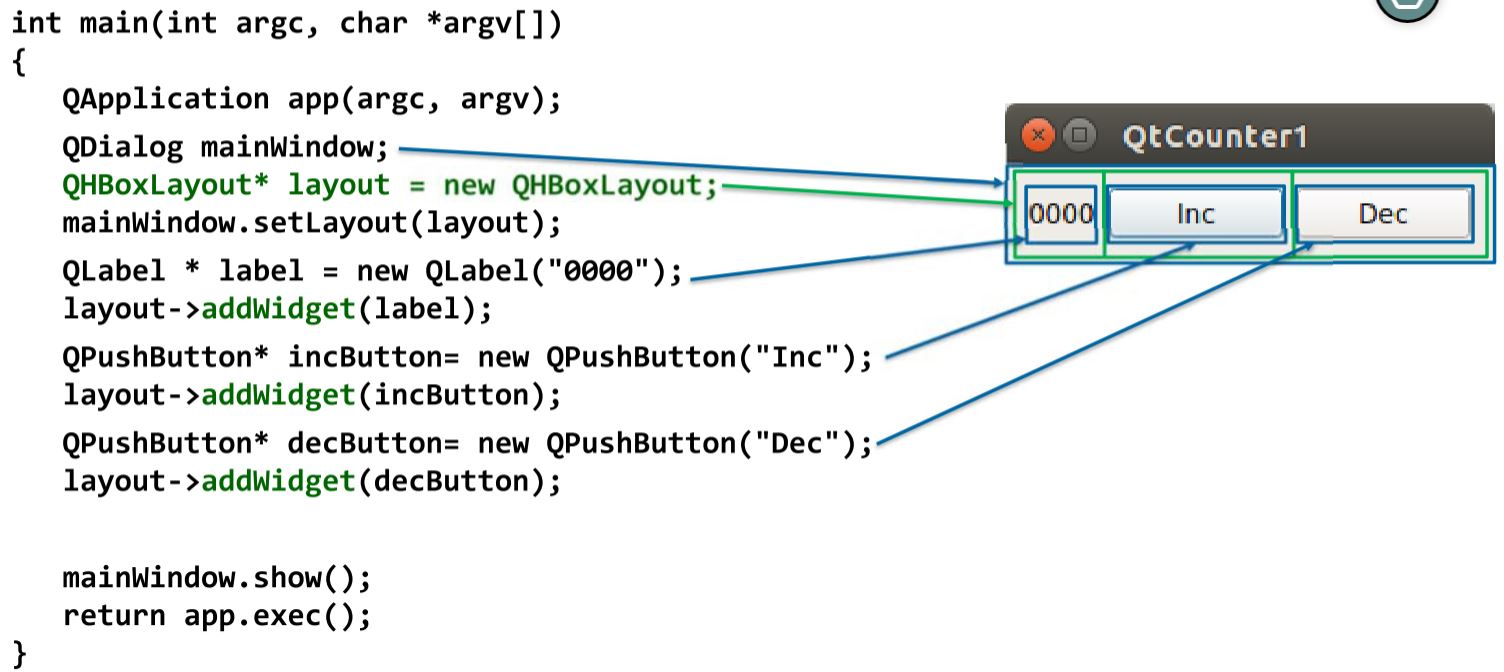
\includegraphics{Figures/QtLayoutManager}}
	\caption[]{Qt Layout Manager}
\end{figure}

Klassen, welche von QLayout ableiten: \\
- QHBoxLayout: Ordnet Elemente horizontal  an \\
- QVBoxLayout: Ordnet Elemente vertikal an \\
- QGridLayout: Ordnet Elemente in einem zweidimensionalen Gitters an. \\
- QFormLayout: Ordnet Elemente in Form von Zeilen an Zeile = QLabel gefolgt von anderem QWidget (z.B. QLineEdit) \\
- QStackedLayout: "Aufeinandergelegte" Widgets (Stapel), nur immer ein Widget ist sichtbar \\
 

Das QLayout-Objekt ist bei einem Parent-Widget zuständig für das Layout (Anordnung) von dessen Child-Widgets:  \\
\textbf{QDialog mainWindow;} \\
\textbf{QVBoxLayout* mainLayout = new QVBoxLayout;} \\
\textbf{mainWindow.setLayout(mainLayout);}
Wird ein child-widget mit addWidget(label) hinzugefügt, dann wird es automatisch mit dem parent Widget verknüpft. 
Das QLayout-Objekt ist selbst ein "Kind" vom "Parent-Widget". Es ist zweckmässig, sich das QLayout-Objekt als ein spezielles Geschwister vorzustellen, das als Kindermädchen ("Nanny") der "Child-Widgets" wirkt. QLayout-Objekte haben nie QWidget-Objekte als eigene Kinder.

Das QLayout-Objekt informiert das "Parent-Widget" automatisch über die Existenz der "Child-Widgets". Das geschieht mittels der addWidget Methode des Layout Managers: \\
\textbf{QLabel * label = new QLabel("0000");}
\textbf{mainLayout‐>addWidget(label);}
Das "Parent-Widget" muss bei den "Child-Widgets" nicht explizit angegeben werden! \\
Layouts können auch verschachtelt werden:
\textbf{QVBoxLayout* mainLayout = new QVBoxLayout;}
\textbf{QHBoxLayout* bottomLayout = new QHBoxLayout;}
\textbf{mainLayout‐>addLayout(bottomLayout);}

\section{Qt Layout Manager}
\begin{figure}[ht]
	\centering
	\adjustbox{width=0.7\textwidth}{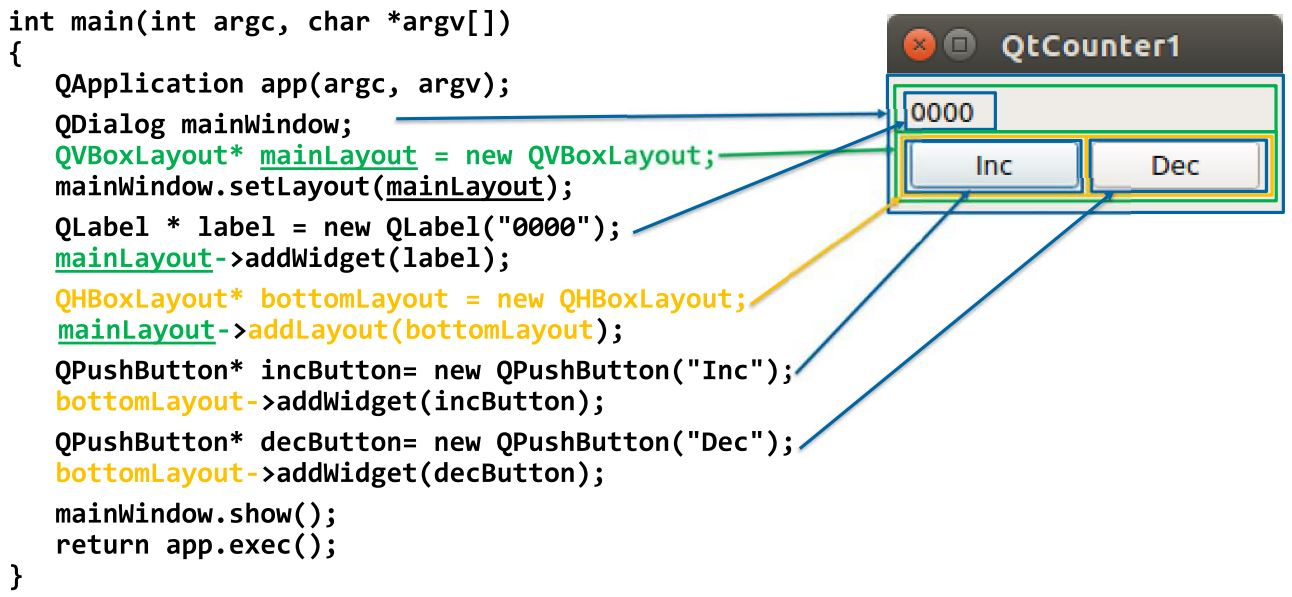
\includegraphics{Figures/layoutmitverschachtelung}}
	\caption[]{Qt Layout: Beispiel mit Verschachtelung}
\end{figure}

\subsection{GUI Erstellung mittels Qt-Creator}

Der Zugriff auf die Widgets:
Widget::Widget(QWidget *parent) :
QWidget(parent),
\textbf{ui(new Ui::Widget)} -> Erstellt ein Layout
{
\textbf{	ui‐>setupUi(this);}
\textbf{	ui‐>lineEdit‐>setText("Test");} -> Setzt den Text in lineEdit Widget
}
Widget::~Widget()
{
\textbf{delete ui;} -> Löscht das Layout
}

ui->lineEdit->setText("Test");

\subsection{Top-Level-Window/Widget}
Definition: Widgets auf der obersten Hierarchiestufe des Widget-Trees.  Widgets ohne Eltern \\
Jedes Widget kann ein "Top-Level-Window" sein
Der Titelbalken ("TitleBar") gehört nicht zu Qt (!), sondern wird vom Betriebssystem erzeugt.
Übliche Widgets für "Top-Level-Windows/Widget":

\textbf{QMainWindow}: Typisch als Applikations-Window (Hauptfenster). Es hat Toolbars und eine Statusbar.

\textbf{QDialog "Popup-Window"}: typisch für Abfragen wie "Soll dies Datei wirklich gelöscht werden?" "Okay", "Abbrechen". \\
Häufig modal, d.h. die Hauptanwendung bleibt blockiert, bis der Dialog beendet ist. Die Standarddialog-Klasse von Qt ist QMessageBox
\textbf{QWidget}: Einfaches Fenster, üblicherweise "non-modal" (d.h nicht blockierend). In den weiteren Beispielen wird meistens QWidget als Top-Level Widget verwendet


\newpage
\section{Qt Widget Collection für Darstellungen (Selbststudium)}


\begin{minipage}{5cm}
	\small{	Single Page Container}
\end{minipage}
\begin{minipage}{5cm}
	\small{Multi Page Container}
\end{minipage}
\begin{minipage}{5cm}
	\small{Button widgets}
\end{minipage}

	\adjustbox{width=5cm}{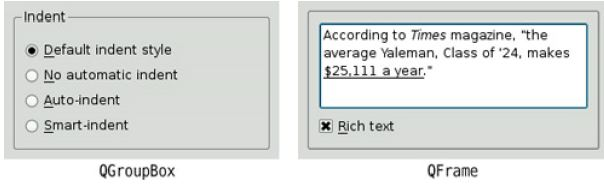
\includegraphics{Figures/scontainer}}
	\adjustbox{width=5cm}{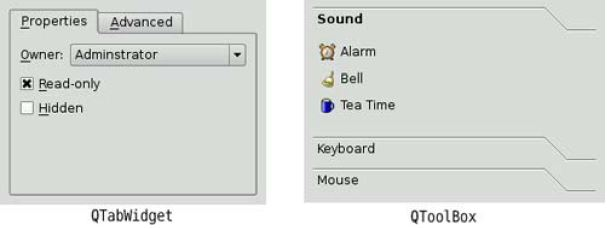
\includegraphics{Figures/mcontainer}} 
	\adjustbox{width=5cm}{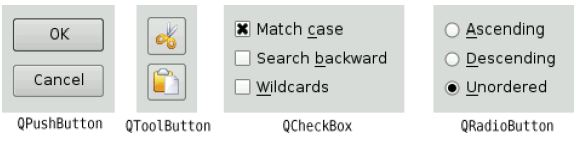
\includegraphics{Figures/buttonwidgets}}
	\\

\begin{minipage}{10cm}
	\small{Input Widget}
\end{minipage}
\begin{minipage}{5cm}
	\small{Color and Font Dialog}
\end{minipage}

	\adjustbox{width=5cm}{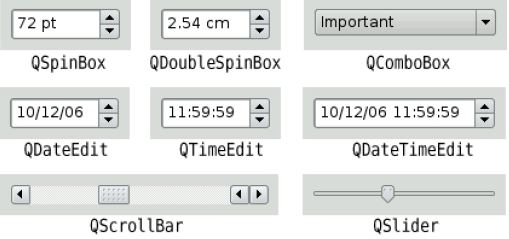
\includegraphics{Figures/inputwidget}}
	\adjustbox{width=5cm}{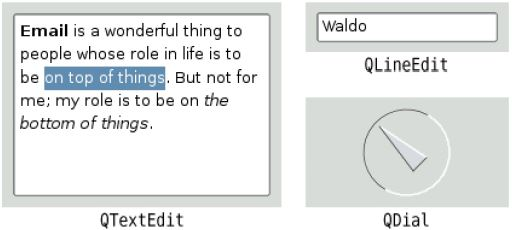
\includegraphics{Figures/inputwidget2}}
	\adjustbox{width=5cm}{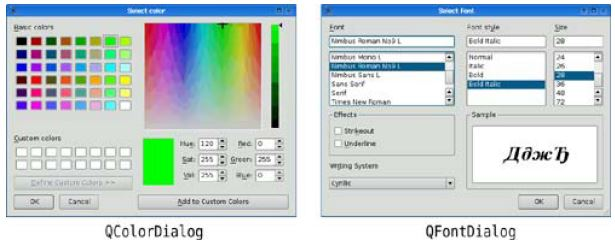
\includegraphics{Figures/cwidget}} \\
	
\begin{minipage}{8cm}
	\small{Item View Widgets}
\end{minipage}
\begin{minipage}{8cm}
	\small{Display Widgets}
\end{minipage}	
	
	\adjustbox{width=8cm}{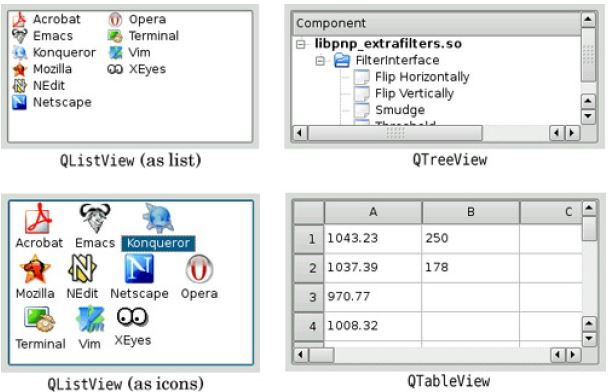
\includegraphics{Figures/vwidget}}
	\adjustbox{width=8cm}{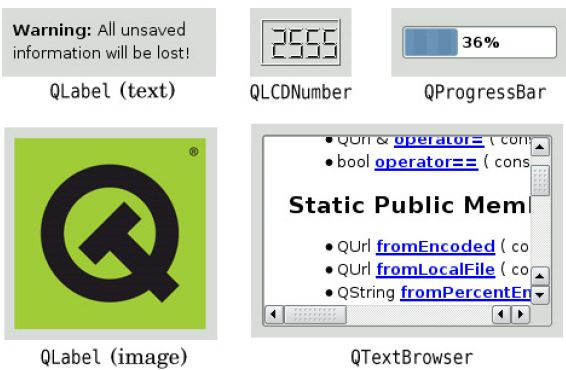
\includegraphics{Figures/dwidget}} \\
	
	\begin{minipage}{8cm}
		\small{File und Print Dialogs}
	\end{minipage}
	\begin{minipage}{8cm}
		\small{Feedback Dialogs}
	\end{minipage}	
	
	\adjustbox{width=8cm}{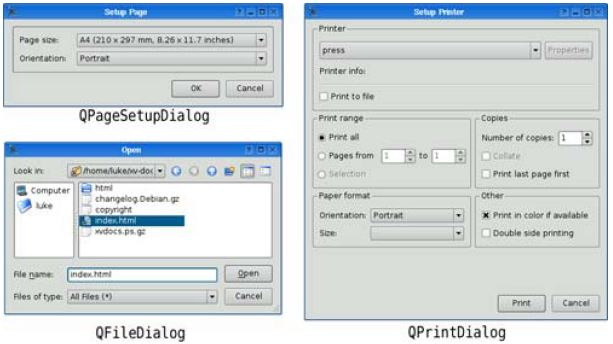
\includegraphics{Figures/pwidget}}
	\adjustbox{width=8cm}{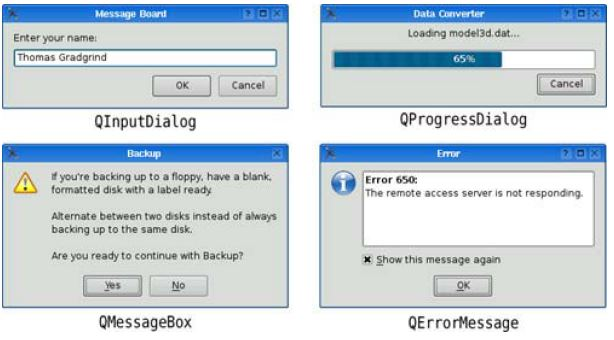
\includegraphics{Figures/fwidget}}

